\section{Auswertung}

\subsection{Messwerte}

Zunächst seien die Messwerte angegeben,
mit denen im Folgenden gerechnet wird.

\begin{table}[H]
  \centering
  \caption{Messwerte zur Bragg-Reflektion.}
  % \label{tab:werte_bragg}
  \begin{tabular}{S[table-format=2.1] c}
  \toprule
  {$\theta_\text{GM} [\si{\degree}]$} &
  {$N$} \\
  \midrule
  \expandableinput{build/table_mess_bragg.tex}
  \bottomrule
  \end{tabular}
\end{table}

\begin{table}[H]
  \centering
  \caption{Messwerte zum Emissionsspektrum.}
  % \label{tab:werte_emissionsspektrum}
  \begin{tabular}{S[table-format=2.1] c | S[table-format=2.1] c | S[table-format=2.1] c | S[table-format=2.1] c}
  \toprule
  {$\theta [\si{\degree}]$} &
  {$N$} &
  {$\theta [\si{\degree}]$} &
  {$N$} &
  {$\theta [\si{\degree}]$} &
  {$N$} &
  {$\theta [\si{\degree}]$} &
  {$N$} \\
  \midrule
  % \expandableinput{build/table_mess_emissionsspektrum.tex}
  \expandableinput{build/table_mess_emissionsspektrum_4col.tex}
  \bottomrule
  \end{tabular}
\end{table}

% –––

\begin{table}[H]
  \centering
  \caption{Messwerte für den Zink-Absorber.}
  % \label{tab:werte_zink}
  \begin{tabular}{S[table-format=2.1] c}
  \toprule
  {$\theta [\si{\degree}]$} &
  {$N$} \\
  \midrule
  \expandableinput{build/table_mess_zink.tex}
  \bottomrule
  \end{tabular}
\end{table}

\begin{table}[H]
  \centering
  \caption{Messwerte für den Gallium-Absorber.}
  % \label{tab:werte_gallium}
  \begin{tabular}{S[table-format=2.1] c}
  \toprule
  {$\theta [\si{\degree}]$} &
  {$N$} \\
  \midrule
  \expandableinput{build/table_mess_gallium.tex}
  \bottomrule
  \end{tabular}
\end{table}

\begin{table}[H]
  \centering
  \caption{Messwerte für den Brom-Absorber.}
  % \label{tab:werte_brom}
  \begin{tabular}{S[table-format=2.1] c}
  \toprule
  {$\theta [\si{\degree}]$} &
  {$N$} \\
  \midrule
  \expandableinput{build/table_mess_brom.tex}
  \bottomrule
  \end{tabular}
\end{table}

\begin{table}[H]
  \centering
  \caption{Messwerte für den Rubidium-Absorber.}
  % \label{tab:werte_rubidium}
  \begin{tabular}{S[table-format=2.1] c}
  \toprule
  {$\theta [\si{\degree}]$} &
  {$N$} \\
  \midrule
  \expandableinput{build/table_mess_rubidium.tex}
  \bottomrule
  \end{tabular}
\end{table}

\begin{table}[H]
  \centering
  \caption{Messwerte für den Strontium-Absorber.}
  % \label{tab:werte_strontium}
  \begin{tabular}{S[table-format=2.1] c}
  \toprule
  {$\theta [\si{\degree}]$} &
  {$N$} \\
  \midrule
  \expandableinput{build/table_mess_strontium.tex}
  \bottomrule
  \end{tabular}
\end{table}

\begin{table}[H]
  \centering
  \caption{Messwerte für den Zirkonium-Absorber.}
  % \label{tab:werte_zirkonium}
  \begin{tabular}{S[table-format=2.1] c}
  \toprule
  {$\theta [\si{\degree}]$} &
  {$N$} \\
  \midrule
  \expandableinput{build/table_mess_zirkonium.tex}
  \bottomrule
  \end{tabular}
\end{table}


\subsection{Überprüfung der Bragg-Bedingung}
\label{sec:auswertung:bragg}

Gemäß der \hyperref[eqn:BraggBedingung]{Bragg-Bedingung} wird erwartet,
dass das gemessene Intensitätsmaximum
($\theta_\text{B, exp} = \SI{28.2}{\degree}$ bzw. $N = \num{218}$)
unter einem der Glanzwinkel auftritt.
In \autoref{fig:plot_bragg} ist gezeigt,
dass diese Annahme zutrifft;
die Abweichung beträgt nur $\SI{0.2}{\degree}$.
% 1:1 Übereinstimmung mit YanickKi

\begin{figure}
    \centering
    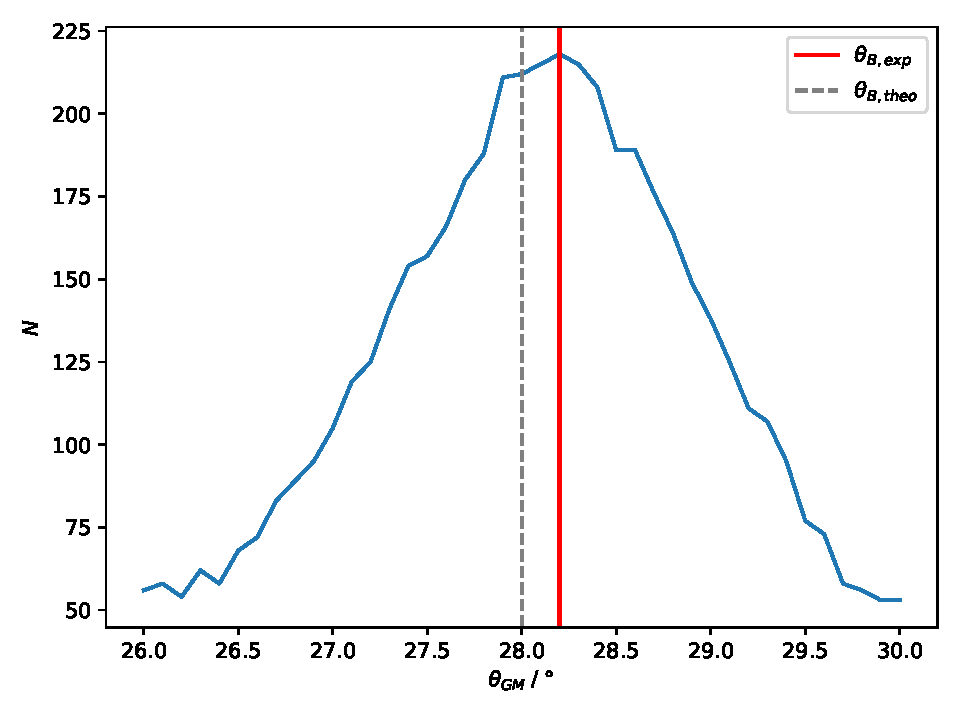
\includegraphics[width=\textwidth]{build/plot_bragg.pdf}
    \caption{Zählrate in Abhängigkeit vom Winkel des Geiger-Müller-Zählrohrs.}
    \label{fig:plot_bragg}
\end{figure}


\subsection{Analyse eines Emissionsspektrums der Kupfer-Röntgenröhre}
\label{sec:auswertung:emissionsspektrum}

In \autoref{fig:emissionsspektrum} ist das Emissionsspektrum der verwendeten Röntgenröhre aufgetragen.
Hervorgehoben sind auch die $K_\alpha$- bzw. $K_\beta$-Kanten
sowie die jeweilige Halbwertsbreite.

\begin{figure}
    \centering
    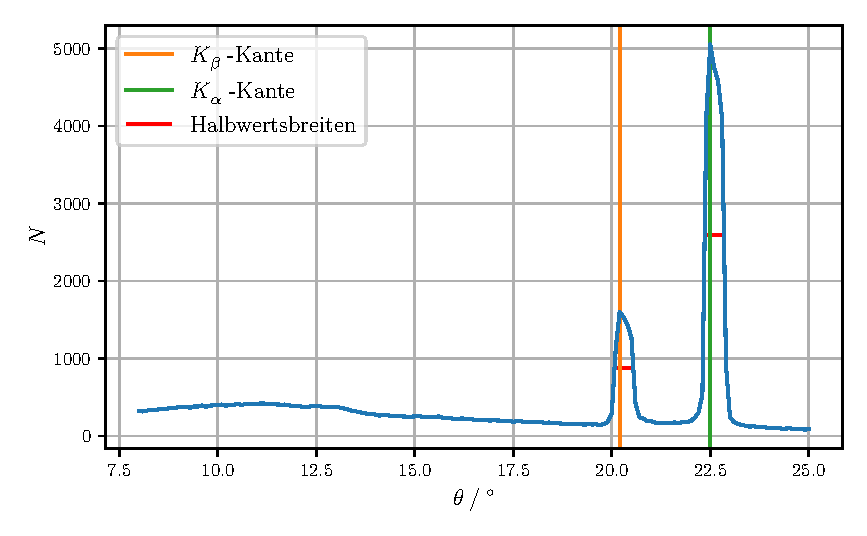
\includegraphics[width=\textwidth]{build/plot_emissionsspektrum.pdf}
    \caption{Das Emissionsspektrum der Kupfer-Röntgenröhre.}
    \label{fig:emissionsspektrum}
\end{figure}

Über den gesamten Messbereich verläuft das \hyperref[sec:theorie:bremsspektrum]{kontinuierliche Bremsspektrum}.
Zudem finden sich zwei Kanten des \hyperref[sec:theorie:char_spektrum]{charakteristischen Spektrums},
deren Intensitätsmaxima mithilfe von \texttt{scipy.signal.find\_peaks} bestimmt wurden.
Sie liegen bei
\begin{align*}
    % 1:1 Übereinstimmung mit YanickKi
    \theta_{K_\alpha} &= \SI{22.5}{\degree} \\
    \theta_{K_\beta}  &= \SI{20.2}{\degree} \; .
\end{align*}


Die Halbwertsbreiten lassen sich mit \texttt{scipy.signal.peak\_widths} finden:
\begin{align*}
    % Erste Abweichung von YanickKi; dort jeweils 0.6°.
    % Unsere mit scipy berechneten Werte sind vmtl. genauer.
    \symup{\Delta}\theta_{K_\alpha} &= \SI{0.490}{\degree} \\
    \symup{\Delta}\theta_{K_\beta}  &= \SI{0.476}{\degree} \; .
\end{align*}


Aus der \hyperref[eqn:BraggBedingung]{Bragg-Bedingung} können nun
die Wellenlänge \hyperref[eqn:lambda_to_E]{und somit die Energie} eines Röntgenquants bestimmt werden.
Die Energien für die Peaks ergeben sich zu
\begin{align*}
    % nahezu identisch mit YanickKi
    E_{K_\alpha} &=  \SI{8.04}{\kilo\electronvolt} \\
    E_{K_\beta}  &=  \SI{8.91}{\kilo\electronvolt} \; .
\end{align*}

Die Energiedifferenzen über die Halbwertsbreiten sind
\begin{align*}
    % Signifikante Abweichungen von YanickKi; siehe oben.
    \symup{\Delta}E_{K_\alpha} &= \SI{0.164}{\kilo\electronvolt} \\
    \symup{\Delta}E_{K_\beta}  &= \SI{0.199}{\kilo\electronvolt} \; .
\end{align*}


Das Auflösungsvermögen ist definiert als
\begin{equation*}
    A = \frac{E}{\symup{\Delta}E}
\end{equation*}
und kann aus den gerade gewonnen Werten zu
\begin{align*}
    A_{K_\alpha} &= \num{48.92} \\
    A_{K_\beta}  &= \num{44.85} \\
\end{align*}
bestimmt werden.
% TODO: Versuchsanleitung: Wie genau ist diese Angabe? Ist es sinnvoll den statistischen Fehler zu bestimmen?


% Mit Hilfe der Gleichungen \eqref{eqn:si1},\eqref{eqn:si2} und \eqref{eqn:si3}…
Mit dem (theoretischen) Literaturwert $E_\text{abs} = \SI{8987.96(15)}{\electronvolt}$ \cite{eabs},
der Rydberg-Energie $R_\infty$ und der Kernladungszahl $Z_\text{Kupfer} = 29$ werden die Abschirmkonstanten
\begin{align*}
    \sigma_1 &= \num{3.298(21)} \\ % ✓ Mampfzwerg, YanickKi
    \sigma_2 &= \num{12.34(13)} \\ % 12.2 Mampfzwerg, 12.30 YanickKi
    \sigma_3 &= \num{22.0(7)}   \\ % 2.9 Mampfzwerg, 21.96 Jean1995 (lit), 22.29 YanickKi
\end{align*}
berechnet.
% TODO: Dazu wurden die Gleichungen XY verwendet.
% \autoref{eqn:SigmaK}
% TODO: Abweichung von den Literaturwerten, siehe https://docs.google.com/viewer?url=https://raw.githubusercontent.com/Jean1995/Praktikum/master/Protokolle_Fertig/V602.pdf


\subsection{Analyse der Absorptionsspektren}
\label{sec:auswertung:absorptionsspektren}

Schließlich sollen die Absorptionsspektren verschiedener Absorbermaterialien analysiert werden.
Dazu wird wieder die Zählrate $N$ gegen den Winkel $\theta$ aufgetragen
und ein näherungsweise linearer Abschnitt als Absorptionskante identifiziert.
Aus dem Winkel in der Mitte dieser kann dann wie zuvor
über die Zusammenhänge von
\hyperref[eqn:BraggBedingung]{Winkel und Wellenlänge (Bragg)} sowie
\hyperref[eqn:lambda_to_E]{Wellenlänge und Energie}
die Absorptionsenergie bestimmt werden.

\subsubsection{Zink}

\begin{figure}[H]
    \centering
    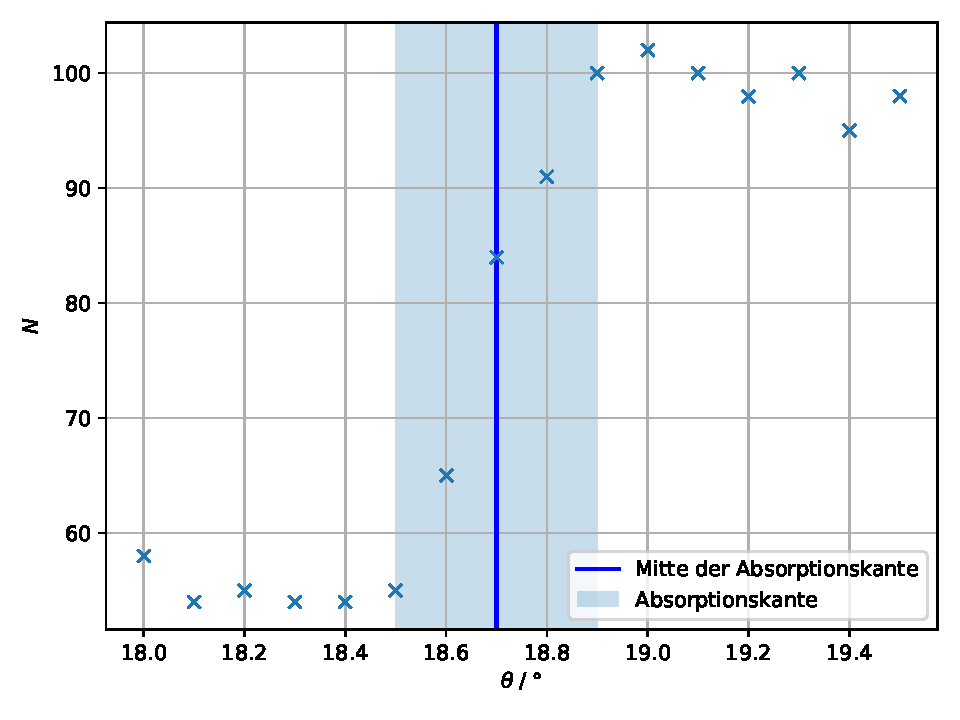
\includegraphics[width=\textwidth]{build/plot_zink.pdf}
    \caption{Absorptionsspektrum von Zink.}
    \label{fig:zink}
\end{figure}

Die Mitte der abgelesenen Absorptionskante liegt bei $\SI{18.7}{\degree}$.
Die Absorptionsenergie beträgt demnach $E_\text{Zink} = \SI{9.601}{\kilo\electronvolt}$.
Die Abschirmkonstante ist $\sigma_{K, \text{Zink}} = \num{3.64}$.

\subsubsection{Gallium}

\begin{figure}[H]
    \centering
    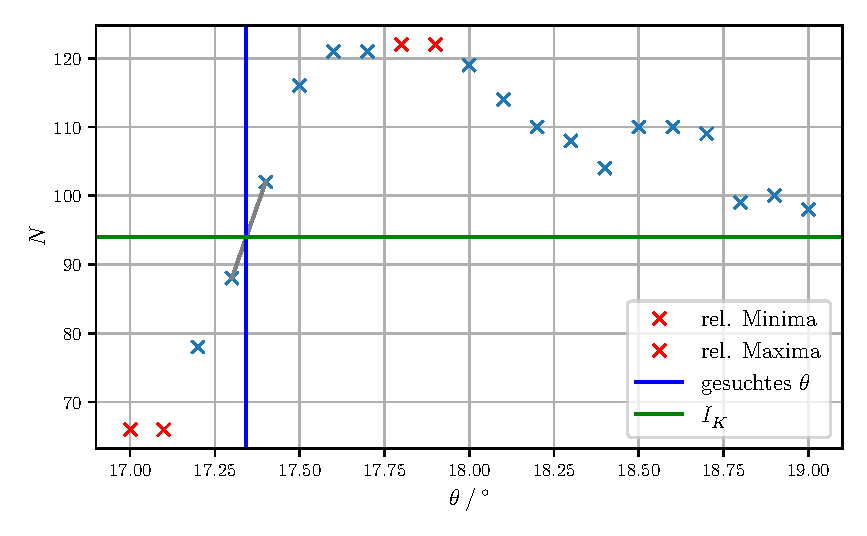
\includegraphics[width=\textwidth]{build/plot_gallium.pdf}
    \caption{Absorptionsspektrum von Gallium.}
    \label{fig:gallium}
\end{figure}

Die Mitte der abgelesenen Absorptionskante liegt bei $\SI{17.35}{\degree}$.
Die Absorptionsenergie beträgt demnach $E_\text{Gallium} = \SI{10.322}{\kilo\electronvolt}$.
Die Abschirmkonstante ist $\sigma_{K, \text{Gallium}} = \num{3.68}$.

\subsubsection{Brom}

\begin{figure}[H]
    \centering
    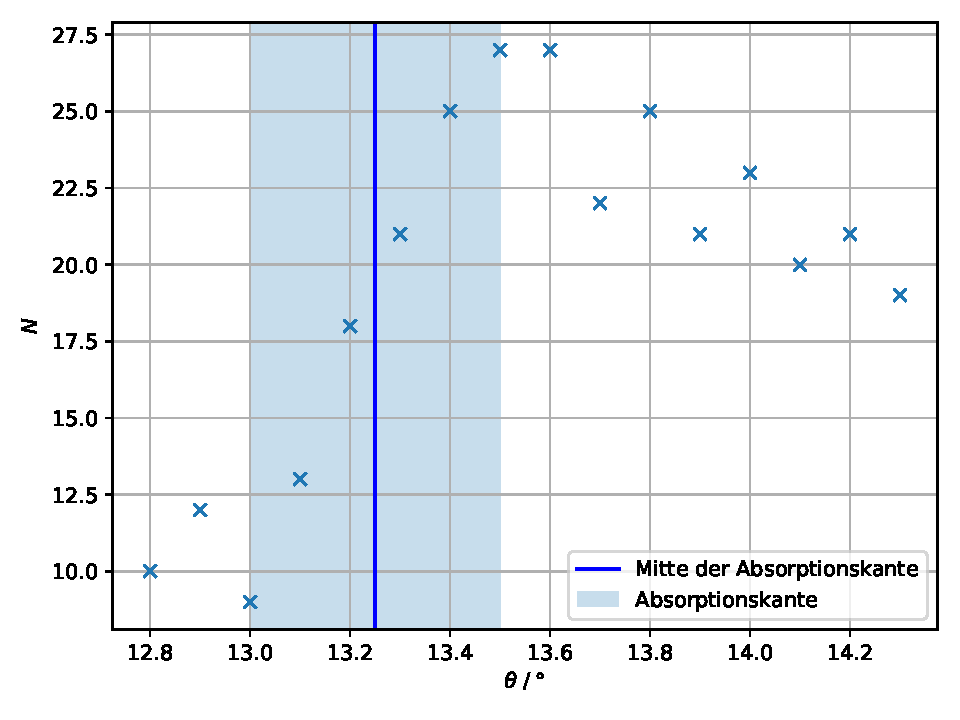
\includegraphics[width=\textwidth]{build/plot_brom.pdf}
    \caption{Absorptionsspektrum von Brom.}
    \label{fig:brom}
\end{figure}

Die Mitte der abgelesenen Absorptionskante liegt bei $\SI{13.25}{\degree}$.
Die Absorptionsenergie beträgt demnach $E_\text{Brom} = \SI{13.430}{\kilo\electronvolt}$.
Die Abschirmkonstante ist $\sigma_{K, \text{Brom}} = \num{3.90}$.

\subsubsection{Rubidium}

\begin{figure}[H]
    \centering
    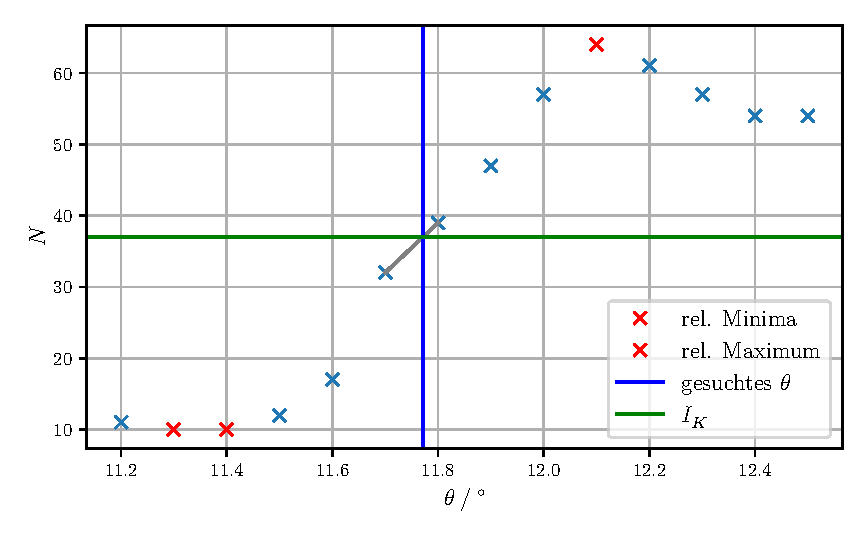
\includegraphics[width=\textwidth]{build/plot_rubidium.pdf}
    \caption{Absorptionsspektrum von Rubidium.}
    \label{fig:rubidium}
\end{figure}

Die Mitte der abgelesenen Absorptionskante liegt bei $\SI{11.75}{\degree}$.
Die Absorptionsenergie beträgt demnach $E_\text{Rubidium} = \SI{15.115}{\kilo\electronvolt}$.
Die Abschirmkonstante ist $\sigma_{K, \text{Rubidium}} = \num{4.05}$.

\subsubsection{Strontium}

\begin{figure}[H]
    \centering
    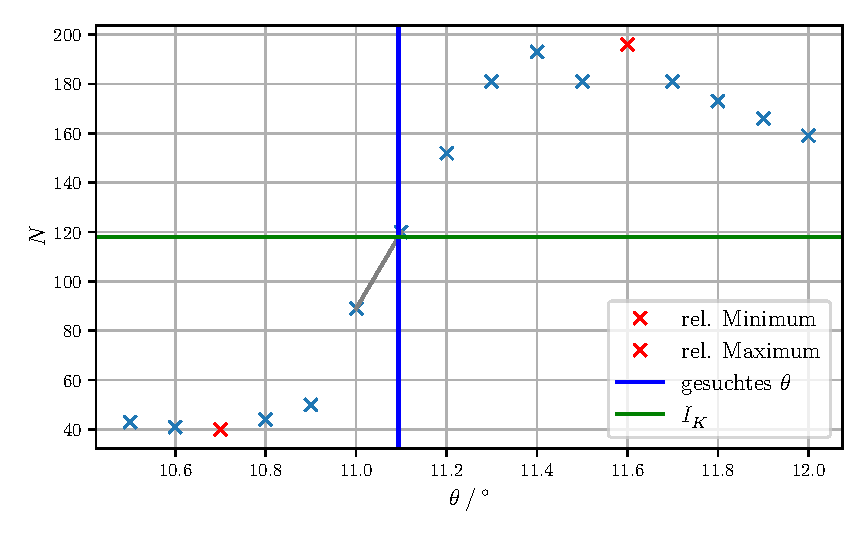
\includegraphics[width=\textwidth]{build/plot_strontium.pdf}
    \caption{Absorptionsspektrum von Strontium.}
    \label{fig:strontium}
\end{figure}

Die Mitte der abgelesenen Absorptionskante liegt bei $\SI{11.1}{\degree}$.
Die Absorptionsenergie beträgt demnach $E_\text{Strontium} = \SI{15.988}{\kilo\electronvolt}$.
Die Abschirmkonstante ist $\sigma_{K, \text{Strontium}} = \num{4.13}$.

\subsubsection{Zirkonium}

\begin{figure}[H]
    \centering
    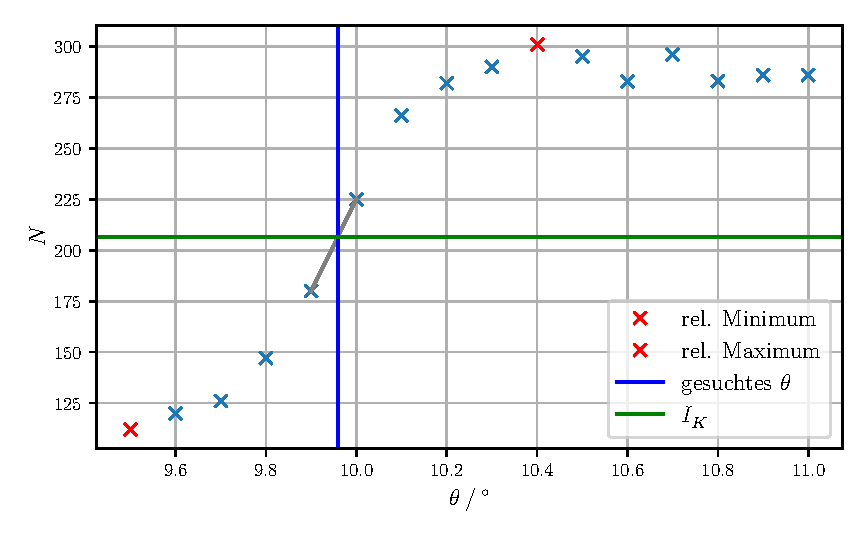
\includegraphics[width=\textwidth]{build/plot_zirkonium.pdf}
    \caption{Absorptionsspektrum von Zirkonium.}
    \label{fig:zirkonium}
\end{figure}

Die Mitte der abgelesenen Absorptionskante liegt bei $\SI{9.95}{\degree}$.
Die Absorptionsenergie beträgt demnach $E_\text{Zirkonium} = \SI{17.814}{\kilo\electronvolt}$.
Die Abschirmkonstante ist $\sigma_{K, \text{Zirkonium}} = \num{4.29}$.


\newpage
\subsection{Moseley'sches Gesetz}
\label{sec:auswertung:moseley}

Mit den gerade gewonnenen Daten soll zuletzt das Moseley'sche Gesetz überprüft werden.
Dazu wird \autoref{eqn:Moseley} zu einer Geradengleichung umgeformt:
\begin{align*}
    E_\text{K} &= R h (z - \sigma)^2 \\
    \Leftrightarrow
    \sqrt{E_\text{K}} &= \underbrace{\sqrt{R h}}_a \cdot z - \underbrace{\sqrt{R h} \sigma_k}_b \; .
\end{align*}

\begin{figure}
    \centering
    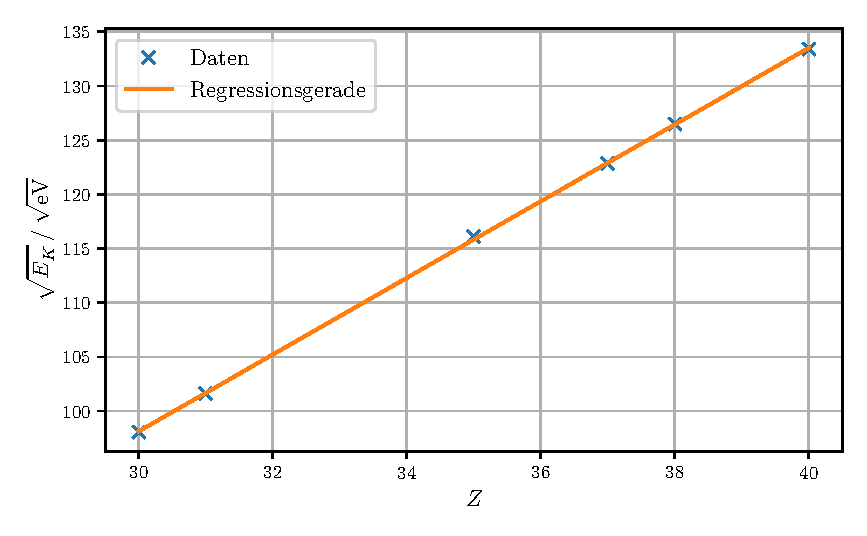
\includegraphics[width=\textwidth]{build/plot_moseley.pdf}
    \caption{Verhältnis von Absorptionsenergien zu Kernladungszahlen mit Regressionsgerade.}
    \label{fig:moseley_regression}
\end{figure}

Mithilfe von linearer Regression werden die Parameter zu
\begin{align*}
    a &= \SI{3.550(8)}{\sqrt{\electronvolt}} \\
    b &= \SI{-8.46(28)}{\sqrt{\electronvolt}} \\
\end{align*}
bestimmt.
Daraus lassen sich die Rydbergenergie
% \begin{align*}
%     R_y &= a^2 = \SI{12.60(6)}{\electronvolt} \\
%     \intertext{und die Rydbergfrequenz}
%     R &= \frac{a^2}{h} = \SI{3.05}{\peta\hertz}
% \end{align*}
\[ R_y = a^2 = \SI{12.60(6)}{\electronvolt} \]
und die Rydbergfrequenz
\[ R = \frac{a^2}{h} = \SI{3.05}{\peta\hertz} \]
errechnen.
